\documentclass[conference]{IEEEtran}
\IEEEoverridecommandlockouts
\usepackage{amsmath,amssymb,booktabs,graphicx,listings,xcolor,tikz,url}
\usetikzlibrary{arrows.meta,positioning,fit}
\lstset{basicstyle=\ttfamily\scriptsize,breaklines=true,frame=single,columns=fullflexible,showstringspaces=false}
\begin{document}
\title{An Adaptive Surveillance Framework for Proximity Assessment and Intrusion Monitoring}
\author{\IEEEauthorblockN{Ayati Rauthan, Ireshi Rawat, and Pranav Tawakley}
\IEEEauthorblockA{Computer and Communication Engineering\\
Manipal Institute of Technology, Manipal, India}}
\maketitle
\begin{abstract}
This report describes an LPC1768 proximity-monitoring prototype and a separate laptop prediction experiment. The board measures distance with an HC-SR04, drives an LCD, seven-segment display, buzzer, LEDs, and servo, and shows a PIR status line. The alarm begins at 30 cm and counts each transition into the alarm state. UART0 exports ultrasonic readings for a small ridge-regression model that forecasts range 0.5 s ahead from five past distances. The model is compared with a constant-speed rule. The software workflow has been tested using 1,000 generated readings; no 1,000-row physical board capture has been completed. On 158 held-out generated windows, the learned model had 4.771 cm mean absolute error versus 5.049 cm for constant speed, but missed three warning-zone windows that the baseline did not miss. These are software rehearsal results, not physical safety results.
\end{abstract}
\begin{IEEEkeywords}LPC1768, ultrasonic ranging, intrusion monitoring, UART, ridge regression, prediction\end{IEEEkeywords}
\section{Introduction}
A person can be close to a doorway monitor without approaching it, while another can be farther away and moving toward it. This motivates studying range over time. The present device is a bench prototype. One ultrasonic sensor cannot identify a person, track several objects, or establish a vehicle's path.

The LPC1768 runs the live distance alarm and display. It also sends readings through CN9 to a laptop, where a separate model predicts range 0.5 s ahead. The lab question is whether a learned forecast beats a constant-speed calculation on unseen trials. ML does not run inside the current LPC1768 firmware. Fig.~\ref{fig:architecture} shows both paths.
% Standalone figure body: paste this figure* into another IEEEtran document if needed.
\begin{figure*}[t]
\centering
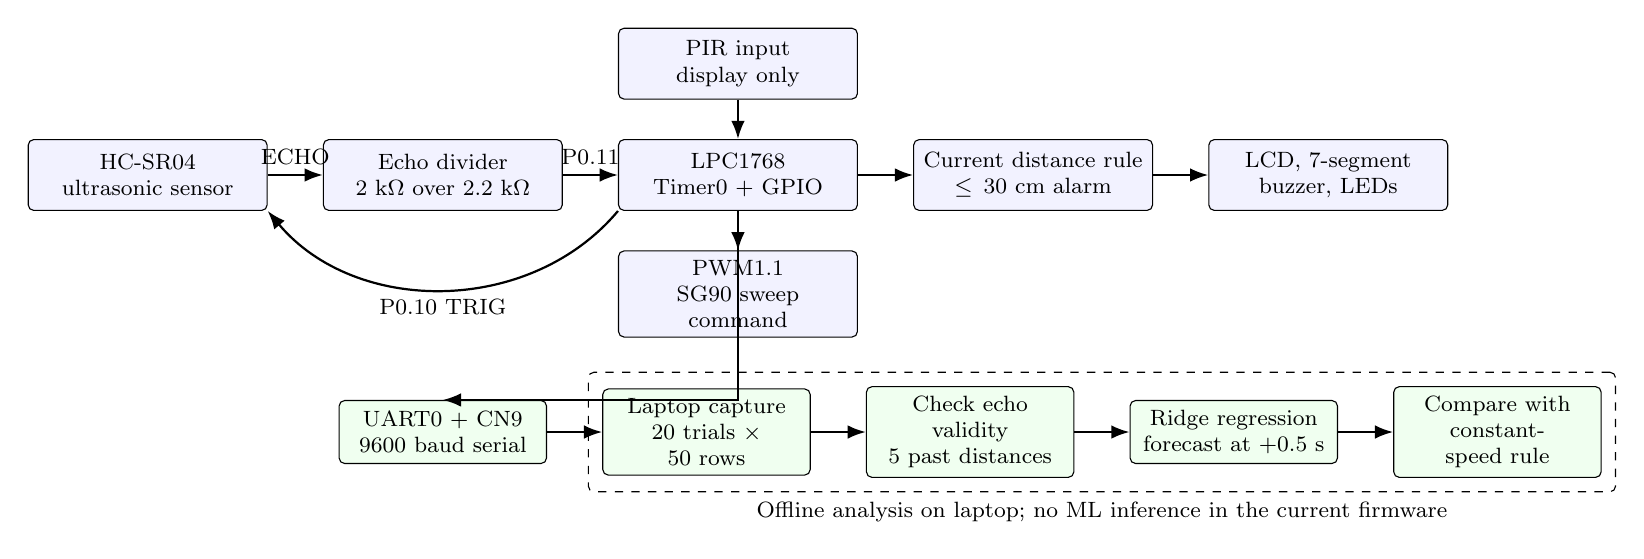
\begin{tikzpicture}[
  font=\footnotesize,
  block/.style={draw,rounded corners=2pt,align=center,minimum height=9mm,text width=28mm,fill=blue!5},
  smallblock/.style={draw,rounded corners=2pt,align=center,minimum height=8mm,text width=24mm,fill=green!6},
  note/.style={draw,dashed,rounded corners=2pt,inner sep=5pt},
  flow/.style={-Latex,thick},
  node distance=5mm and 7mm]
\node[block] (sensor) {HC-SR04\\ultrasonic sensor};
\node[block,right=of sensor] (divider) {Echo divider\\2 k$\Omega$ over 2.2 k$\Omega$};
\node[block,right=of divider] (mcu) {LPC1768\\Timer0 + GPIO};
\node[block,above=of mcu] (pir) {PIR input\\display only};
\node[block,below=of mcu] (servo) {PWM1.1\\SG90 sweep command};
\node[block,right=of mcu] (alarm) {Current distance rule\\$\leq 30$ cm alarm};
\node[block,right=of alarm] (outputs) {LCD, 7-segment\\buzzer, LEDs};
\draw[flow] (sensor) -- node[above]{ECHO} (divider);
\draw[flow] (divider) -- node[above]{P0.11} (mcu);
\draw[flow] (mcu) -- (alarm);
\draw[flow] (alarm) -- (outputs);
\draw[flow] (pir) -- (mcu);
\draw[flow] (mcu) -- (servo);
\draw[flow] (mcu.south west) to[out=230,in=310] node[below]{P0.10 TRIG} (sensor.south east);
\node[smallblock,below=24mm of divider] (uart) {UART0 + CN9\\9600 baud serial};
\node[smallblock,right=of uart] (capture) {Laptop capture\\20 trials $\times$ 50 rows};
\node[smallblock,right=of capture] (clean) {Check echo validity\\5 past distances};
\node[smallblock,right=of clean] (model) {Ridge regression\\forecast at +0.5 s};
\node[smallblock,right=of model] (compare) {Compare with\\constant-speed rule};
\draw[flow] (mcu.south) |- (uart.north);
\draw[flow] (uart) -- (capture);
\draw[flow] (capture) -- (clean);
\draw[flow] (clean) -- (model);
\draw[flow] (model) -- (compare);
\node[note,fit=(capture)(clean)(model)(compare),label={[font=\footnotesize]below:Offline analysis on laptop; no ML inference in the current firmware}] {};
\end{tikzpicture}
\caption{Detailed architecture of the present prototype. The upper path is the live embedded warning system. The lower path is the separate data-capture and prediction experiment. The dataset currently committed to the repository is generated practice data; physical UART capture is still pending.}
\label{fig:architecture}
\end{figure*}

\section{Literature Review}
Recent warning research uses richer motion and scene information than our one-range prototype. Jiao et al. study trajectory-based traffic conflicts \cite{jiao2025}. Zhao et al. define collision regions from spatial state \cite{zhao2024}, while Han et al. adapt a warning region to road geometry and kinematics \cite{han2025}. These papers motivate an explicit region of concern, but their traffic findings do not transfer to our bench setup.

Driver-warning research examines response behavior, timing, and unnecessary alerts \cite{shao2023,bao2024,xie2024,fu2025,olufowobi2025,xu2024,yang2025}. Pedestrian near-miss analysis uses trajectories and surrogate safety measures \cite{ahsan2024}. Westhofen et al. review criticality metrics \cite{westhofen2023}. We therefore report both forecast error and missed 30 cm zone windows; mean error alone can hide late warnings. Richer systems combine inertial and ultrasonic measurements \cite{hybrid2024}, use acoustic arrays \cite{izquierdo2024}, or combine radio sensing with ML \cite{cardenas2024}. Our hardware does none of those tasks.
\subsection{Research gap}
The narrow lab question is how a learned short-range forecast compares with a simple motion forecast when both receive the same ultrasonic history. Current ML results use only generated practice data. The PIR input has been unreliable in the team's tests. One ultrasonic range also lacks identity and lateral position, so this is not a validated real-world near-miss detector.
\section{Methodology}
\subsection{Hardware and live behavior}
The ALS LPC1768 trainer uses an HC-SR04, an ECHO voltage divider, SG90 servo, LCD, seven-segment display, buzzer, and LEDs. Timer0 measures ECHO pulse width. Firmware sends a 12 microsecond trigger, waits at most 30 ms for an echo transition, and converts a valid pulse using approximately $d_{\rm cm}=t_{\rm echo,\mu s}/58$. Readings outside 2--400 cm are invalid. The loop aims for one reading every 100 ms.

PWM1.1 commands pulses from 1000 to 2000 microseconds in 10 microsecond steps, updated about every 20 ms. These are commanded widths; actual endpoint angles have not been measured. If the ultrasonic head rotates, successive readings may come from different directions. For motion prediction the head must be fixed, even if the unloaded servo keeps moving.

The live alarm is off above 30 cm or on an invalid echo. It is continuous from 15 to 30 cm and pulses 80 ms on, 120 ms off below 15 cm. LEDs follow the buzzer. LCD line one counts changes from alarm-off to alarm-on, not individual beeps. Line two shows PIR state after a 60 s warm-up. PIR is excluded from alarm decisions and ML features. The seven-segment display shows range or dashes for an invalid echo.
\begin{table}[t]\caption{Signals used by the current firmware}\label{tab:pins}\centering\footnotesize
\begin{tabular}{lll}\toprule
Signal & MCU function & Trainer connection\\\midrule
HC-SR04 TRIG & P0.10 GPIO & CN6 pin 7\\
HC-SR04 ECHO, divided & P0.11 GPIO & CN6 pin 8\\
Servo command & P2.0 PWM1.1 & CN6 pin 1\\
PIR status & P2.2 or P2.3 & CN6 pin 23 or 24\\
Serial telemetry & P0.2 TXD0 & CN9 RS232\\
LCD & P0.23--P0.28 & CND--CNAD ribbon\\
Buzzer & P1.23 & CNB--CNA5 jumper\\\bottomrule
\end{tabular}\end{table}
The nominal 5 V ECHO passes through two 1 k$\Omega$ resistors in series, then a node with 2.2 k$\Omega$ to ground. A 5 V HIGH gives about $5(2.2)/(1+1+2.2)=2.62$ V at that node. Sensor and board share ground. Power and jumpers must be checked on the physical trainer.
\subsection{Serial capture}
UART0 emits one line through the board's RS232 converter at 9600 baud, 8N1. Fields are sequence number, board time, distance, validity, commanded servo pulse, and sensor status. An invalid echo has a blank distance. The laptop parser checks record format, packet sequence, and timing. Listing~\ref{lst:uart} shows the core export.
\begin{lstlisting}[language=C,caption={Condensed UART record from main.c.},label={lst:uart}]
uart0_text("DATA,");
uart0_uint(sequence); uart0_char(',');
uart0_uint(time_us / 1000U); uart0_char(',');
if (status == DIST_OK) uart0_uint(distance);
uart0_char(',');
uart0_uint(status == DIST_OK ? 1U : 0U);
uart0_char(',');
uart0_uint(pulse_us); uart0_char(',');
uart0_uint(status); uart0_text("\r\n");
\end{lstlisting}
The planned board capture has 20 five-second trials of 50 readings: five approaches, five walks away, five approaches stopping before the zone, and five pass-bys outside it. The script writes the CSV only after all trials succeed and records a checksum. No physical 1,000-row capture is present. The included file was generated to rehearse the pipeline and labels every row SIMULATED. Its four scenario types have five trials each. The generator adds small range noise, occasional larger errors, and missing echoes; these are software choices, not measurements of the HC-SR04's error distribution.
\subsection{Preprocessing and target}
Rows are grouped by trial and ordered by relative time. Missing echoes remain in the CSV but are excluded from prediction windows. A usable window needs five valid distances about 100 ms apart and a valid label 500 ms after the newest input. Thus $\mathbf{x}_t=[d_t,d_{t-1},d_{t-2},d_{t-3},d_{t-4}]$ and $y_t=d_{t+0.5\,{\rm s}}$. No future reading enters the input. Listing~\ref{lst:window} shows the indexing; the full script also checks blank fields and time tolerance.
\begin{lstlisting}[language=Python,caption={Condensed history construction from train_model.py.},label={lst:window}]
past = trial[index - HISTORY + 1:index + 1]
future = trial[index + HORIZON]
if any(r["valid"] != "1" for r in past):
    continue
if future["valid"] != "1":
    continue
distances = [float(r["distance_cm"])
             for r in reversed(past)]
target = float(future["distance_cm"])
\end{lstlisting}
The Jupyter notebook checks source labels and trial sizes, converts data types, leaves failed echoes missing, summarizes scenarios, and plots predictions.
\subsection{Model and baseline}
The five-input ridge model gives $\hat y_t=b+\sum_{j=0}^{4}w_jd_{t-j}$ and penalizes large weights. Validation trials select a penalty from 0.1, 1, and 10. On the generated dataset the selected penalty was 0.1, with 3.529 cm validation MAE. The fitted coefficients (newest range first) were $b=4.483$ and $\mathbf{w}=(1.705,0.636,0.116,-0.529,-0.964)$. These numbers describe this generated dataset only; they should be refitted after a board capture. A constant-speed baseline extrapolates change over the 0.4 s history by 0.5 s:
\begin{equation}\hat y_t^{\rm base}=\max\{0,d_t+1.25(d_t-d_{t-4})\}.\end{equation}
Predictions are clipped at zero. Both methods use identical histories and labels. The 20 trials split by scenario into 12 training, four validation, and four test trials. Keeping a walk entirely in one set avoids leakage from adjacent, similar readings.
\subsection{Evaluation}
Distance error is $\mathrm{MAE}=N^{-1}\sum_i|\hat y_i-y_i|$. A future zone event means future range is 30 cm or less. We count correct, false, and missed warning windows plus correct nonwarnings on held-out trials. A window is one forecast, not an independent person or collision. Replay lead time is the interval from first forecast warning to later measured zone entry.
\section{Results and Discussion}
\subsection{Data quality}
The generated file has 1,000 rows: 20 trials of 50 readings. It contains 982 valid distances and 18 missing echoes. Skipping histories with an invalid input or label leaves 730 usable windows. The 12/4/4 trial split leaves 158 test windows. Fig.~\ref{fig:quality} shows the notebook summary.
\begin{figure}[t]\centering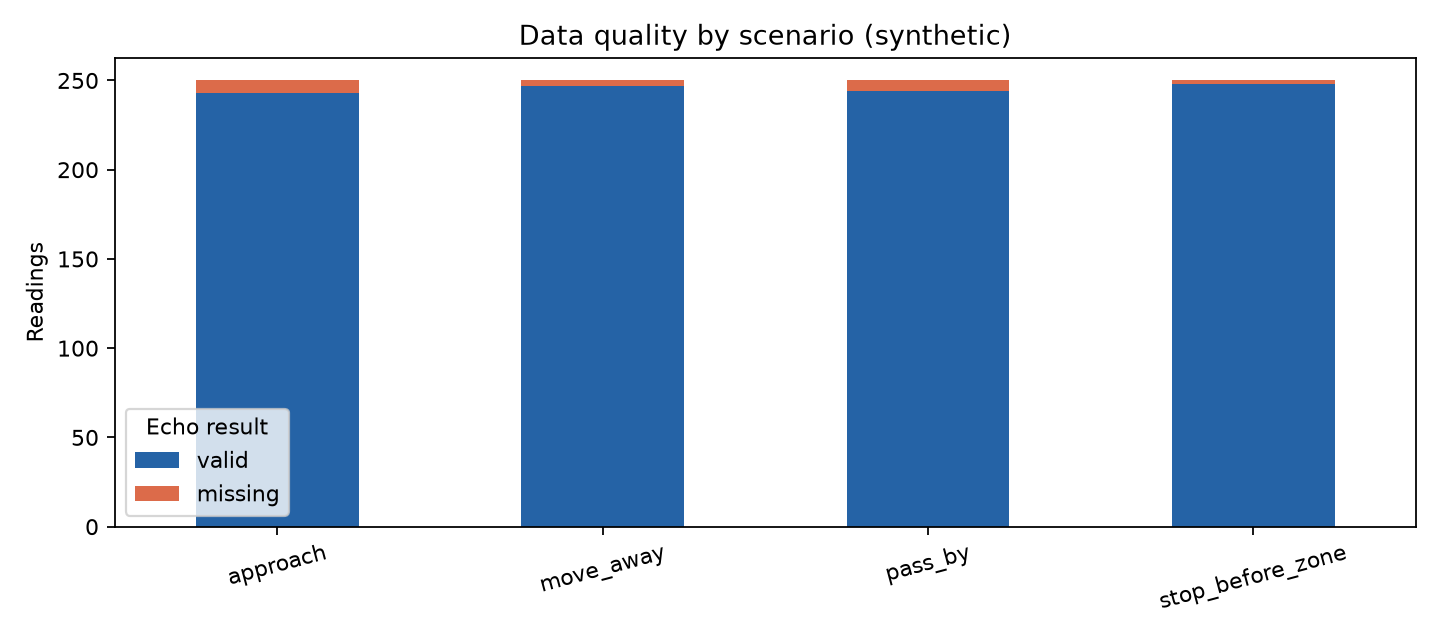
\includegraphics[width=\columnwidth]{images/01_data_quality.png}
\caption{Data-quality summary for generated practice data.}\label{fig:quality}\end{figure}
\subsection{Prediction and warning results}
Table~\ref{tab:results} reports zone decisions as well as error. The learned model reduced overall MAE by 0.278 cm on held-out generated windows. It also missed three zone entries; the baseline missed none. This does not show that ML is safer. Neither method had a false warning window in this small test.
\begin{table}[t]\caption{Held-out generated-data results (158 windows)}\label{tab:results}\centering\footnotesize
\begin{tabular}{lrr}\toprule
Measure & Constant speed & Ridge ML\\\midrule
Mean absolute error (cm) & 5.049 & 4.771\\
Correct warning windows & 15 & 12\\
False warning windows & 0 & 0\\
Missed zone windows & 0 & 3\\
Correct nonwarning windows & 143 & 143\\\bottomrule
\end{tabular}\end{table}
In held-out approach trial 03, a 36 cm reading at 3.3 s led to a learned forecast of 23.9 cm and a warning. Measured range entered the 30 cm zone at 3.5 s, giving 0.2 s lead in that generated example. Held-out pass-by trial 04 stayed at least 58 cm away and produced no replay warning. These are software examples, not observed campus intrusions. Fig.~\ref{fig:traces} shows the trajectories.
\begin{figure}[t]\centering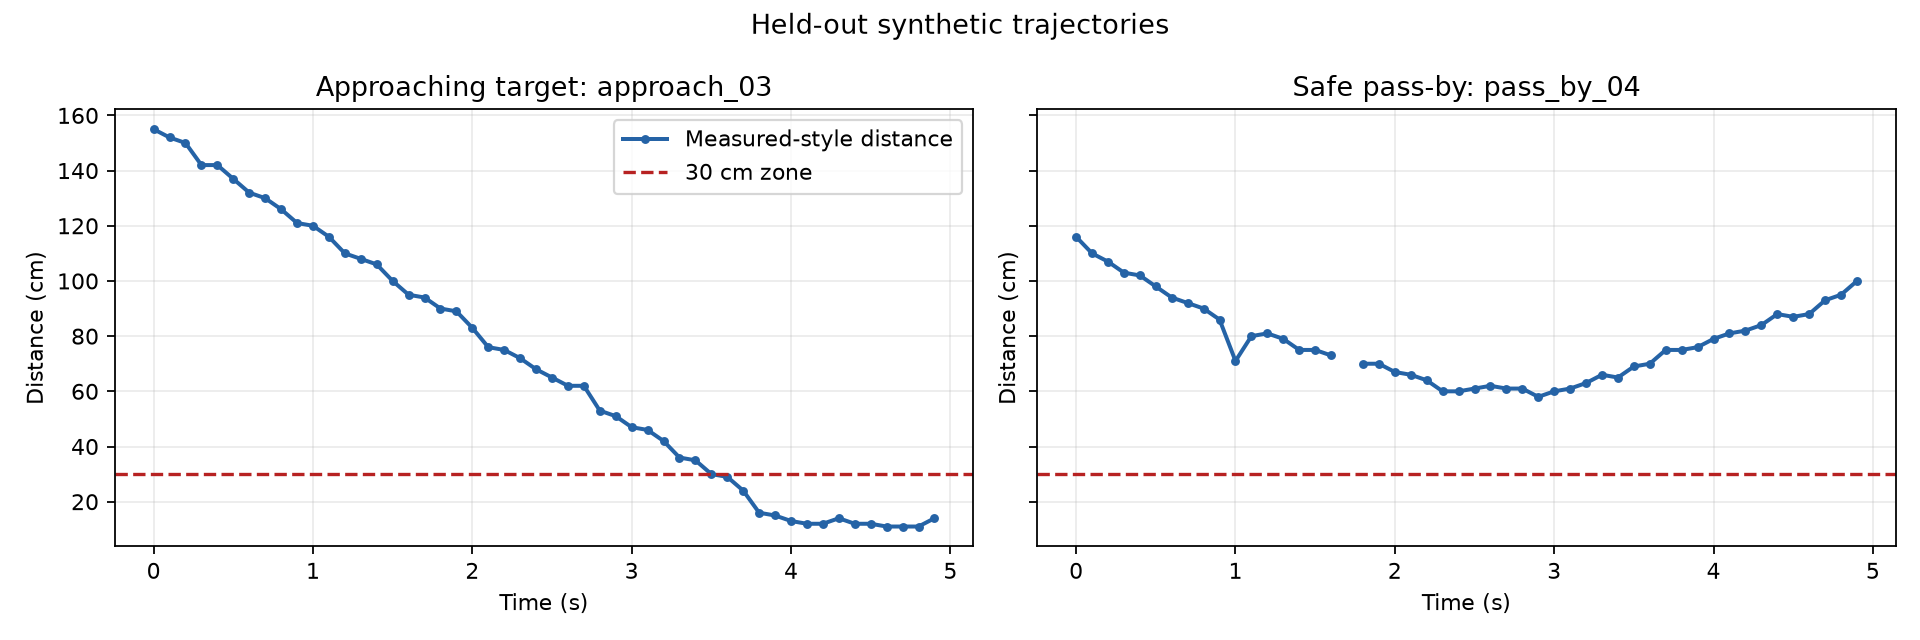
\includegraphics[width=\columnwidth]{images/03_held_out_trajectories.png}
\caption{Held-out generated distance trajectories. The dashed line marks the 30 cm zone.}\label{fig:traces}\end{figure}
On the held-out approach trial, ML error was 4.40 cm, slightly worse than constant speed at 4.15 cm. Lower overall error came from other scenarios. The missed zone windows matter because late warnings are the failure the project aims to avoid.
\subsection{Validation status}
The Python parser, split logic, and trainer passed six local software tests. The modified C source passed a host syntax check using a minimal header stub. Keil compilation of this exact revision, physical UART capture, servo endpoint calibration, and real-data model comparison remain pending. The board alarm uses measured distance; ML appears only in laptop analysis and replay files.
\section{Conclusion}
The framework links an LPC1768 proximity alarm design with a reproducible offline prediction experiment. The additions are serial export, missing-echo handling, whole-trial evaluation, and comparison with a simple speed rule. On generated practice data, ridge regression slightly improved mean distance error but missed more warning-zone windows. The next step is to hold the ultrasonic sensor fixed, collect real UART readings, and repeat the analysis before making physical warning claims.
\begin{thebibliography}{15}
\bibitem{jiao2025} Y. Jiao, S. C. Calvert, S. van Cranenburgh, and H. van Lint, "A unified probabilistic approach to traffic conflict detection," \emph{Analytic Methods in Accident Research}, vol. 45, Art. 100369, 2025, doi: \url{10.1016/j.amar.2024.100369}.
\bibitem{zhao2024} W. Zhao et al., "A spatial-state-based omni-directional collision warning system for intelligent vehicles," \emph{IEEE Trans. Intelligent Transportation Systems}, vol. 25, no. 10, pp. 14344--14358, 2024, doi: \url{10.1109/TITS.2024.3387942}.
\bibitem{han2025} S. Han et al., "Adaptive ROI for collision warning mitigation based on road geometry and kinematics," \emph{IEEE Sensors Journal}, vol. 25, no. 3, pp. 5499--5509, 2025, doi: \url{10.1109/JSEN.2024.3512947}.
\bibitem{shao2023} Y. Shao et al., "Adaptive forward collision warning system for hazmat truck drivers," \emph{Accident Analysis \& Prevention}, vol. 191, Art. 107221, 2023, doi: \url{10.1016/j.aap.2023.107221}.
\bibitem{bao2024} Y. Bao and X. Wang, "Optimization of forward collision warning algorithm considering truck driver response behavior characteristics," \emph{Accident Analysis \& Prevention}, vol. 198, Art. 107450, 2024, doi: \url{10.1016/j.aap.2023.107450}.
\bibitem{xie2024} N. Xie et al., "Personalized forward collision warning model with learning from human preferences," \emph{Accident Analysis \& Prevention}, vol. 208, Art. 107791, 2024, doi: \url{10.1016/j.aap.2024.107791}.
\bibitem{fu2025} Q. Fu et al., "How predictive-forward-collision-warning reduces the collision risk of leading vehicle driver," \emph{Accident Analysis \& Prevention}, vol. 211, Art. 107891, 2025, doi: \url{10.1016/j.aap.2024.107891}.
\bibitem{olufowobi2025} O. Olufowobi et al., "Safety effectiveness of forward collision warning systems in the vehicle fleet: A driving simulation study," \emph{Accident Analysis \& Prevention}, vol. 218, Art. 108078, 2025, doi: \url{10.1016/j.aap.2025.108078}.
\bibitem{ahsan2024} M. J. Ahsan, M. Abdel-Aty, and N. Anwari, "Vehicle-Pedestrian near miss analysis at signalized mid-block crossings," \emph{Journal of Safety Research}, vol. 91, pp. 68--84, 2024, doi: \url{10.1016/j.jsr.2024.08.006}.
\bibitem{hybrid2024} L. Qi, Y. Liu, C. Gao, T. Feng, and Y. Yu, "Hybrid pedestrian positioning system using wearable inertial sensors and ultrasonic ranging," \emph{Defence Technology}, vol. 33, pp. 327--338, 2024, doi: \url{10.1016/j.dt.2023.11.006}.
\bibitem{xu2024} J. Xu and A. R. Bowers, "Hazard warning modalities and timing thresholds for older drivers with impaired vision," \emph{Accident Analysis \& Prevention}, vol. 202, Art. 107599, 2024, doi: \url{10.1016/j.aap.2024.107599}.
\bibitem{yang2025} D. Yang et al., "Drivers' reactions to real-world forward collision warnings," \emph{Accident Analysis \& Prevention}, vol. 210, Art. 107853, 2025, doi: \url{10.1016/j.aap.2024.107853}.
\bibitem{westhofen2023} L. Westhofen et al., "Criticality metrics for automated driving: A review and suitability analysis of the state of the art," \emph{Archives of Computational Methods in Engineering}, vol. 30, pp. 1--35, 2023, doi: \url{10.1007/s11831-022-09788-7}.
\bibitem{cardenas2024} J. D. Cardenas et al., "Experimental evaluation of a head-on collision warning system fusing machine learning and decentralized radio sensing," \emph{IEEE Sensors Journal}, 2024, doi: \url{10.1109/JSEN.2024.3403492}.
\bibitem{izquierdo2024} A. Izquierdo, L. del Val, and J. J. Villacorta, "Pedestrian detection using a MEMS acoustic array mounted on a moving vehicle," \emph{Sensors and Actuators A: Physical}, vol. 376, Art. 115586, 2024, doi: \url{10.1016/j.sna.2024.115586}.
\end{thebibliography}
\end{document}
